\documentclass{classes/report}

\usepackage{enumitem}
\pagestyle{empty}

\begin{document}
% textlint-disable ja-technical-writing/ja-no-mixed-period
基礎電子工学 \ 第5回 \ 課題
% textlint-enable ja-technical-writing/ja-no-mixed-period
\begin{flushright}
    \underline{\ 学籍番号 \ 2397002 \ 氏名 \ 杉本 謙仁 \ }
\end{flushright}

\bigskip

\begin{enumerate}
    \item フェルミ準位の値と温度を適当に決めて,フェルミーディラックの分布関数を描け.
\end{enumerate}

フェルミ準位を $E_F = 1 [\mathrm{eV}]$,温度を $T = 300 [\mathrm{K}]$ とする.

% ./figures/fermi-dirac.jpgを挿入
\begin{figure}[htbp]
    \centering
    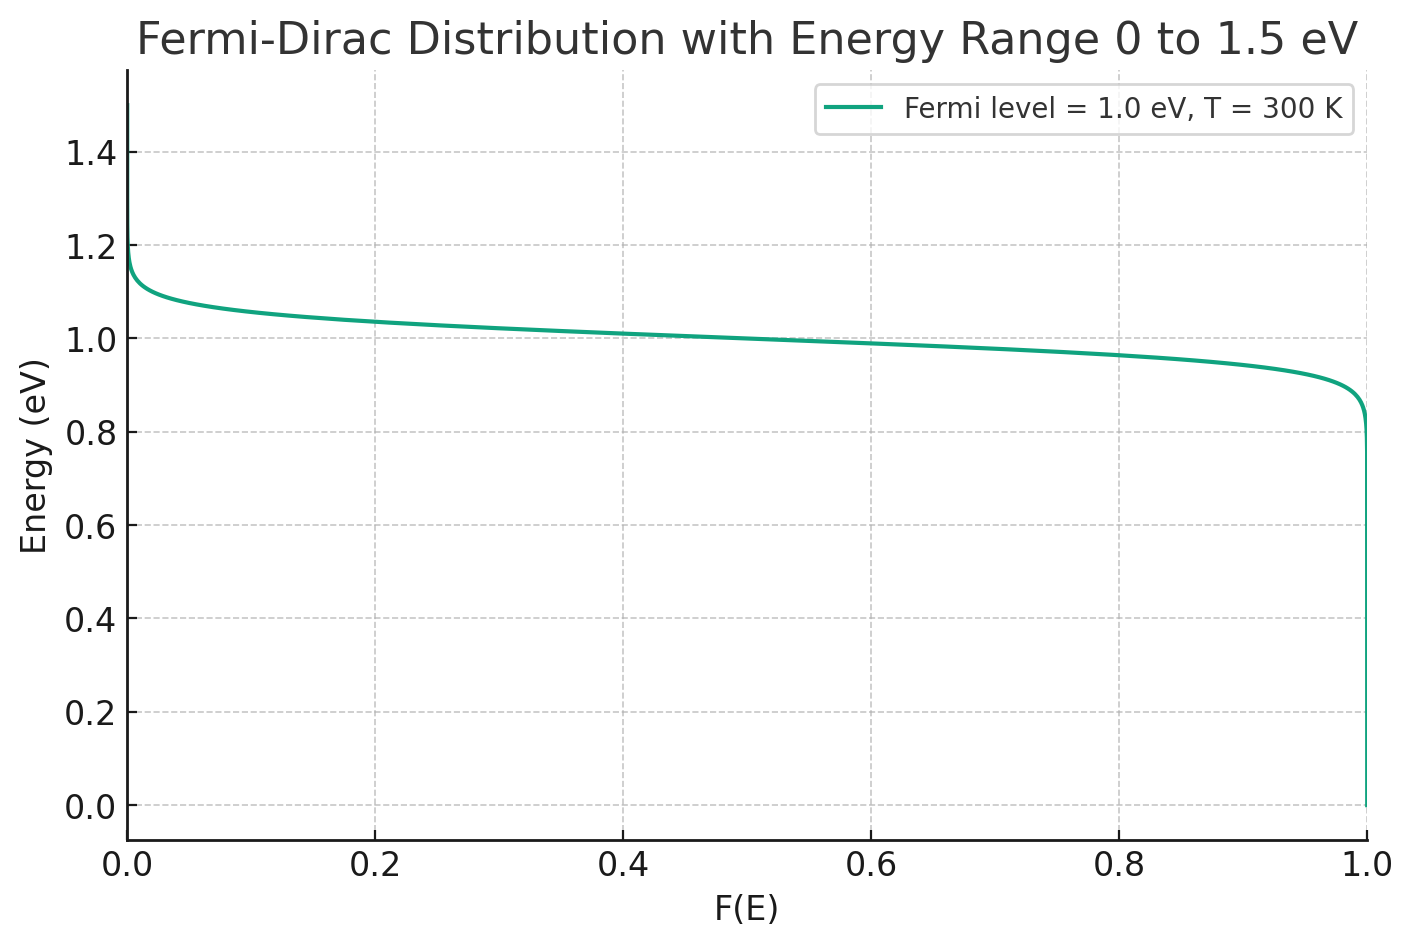
\includegraphics[width=0.8\linewidth]{./figures/fermi-dirac.jpg}
    \caption{フェルミーディラックの分布関数}
\end{figure}

\bigskip

\begin{enumerate}[resume]
    \item 室温でのn型半導体の電子密度が$5\times 10^{21} [m^{-3}]$であった.正孔密度を求めよ.ただし,真性キャリア
    密度は $1\times 10^{16} [m^{-3}]$とする.
\end{enumerate}

\( n \) 型半導体における電子の密度 \( n \) と正孔の密度 \( p \) と真性キャリア密度 \( n_i \) の関係は次のように表される.

\[ n \cdot p = n_i^2 \]    

ここで,\( n \) は\( 5 \times 10^{21} \, \text{m}^{-3} \),\( n_i \) は \( 1 \times 10^{16} \, \text{m}^{-3} \).
以上より,

\[ p = \frac{n_i^2}{n} = \frac{(1 \times 10^{16} \, \text{m}^{-3})^2}{5 \times 10^{21} \, \text{m}^{-3}} = \frac{1 \times 10^{32} \, \text{m}^{-6}}{5 \times 10^{21} \, \text{m}^{-3}} = 2 \times 10^{10} \, \text{m}^{-3} \]

したがって,正孔の密度 \( p \) は \(2 \times 10^{10} \, \text{m}^{-3}\) .


\end{document}